\documentclass[letterpaper,10pt]{article}

\usepackage{titling}
\usepackage{listings}
\usepackage{url}
\usepackage{setspace}
\usepackage{subfig}
\usepackage{sectsty}
\usepackage{pdfpages}
\usepackage{colortbl}
\usepackage{multirow}
\usepackage{relsize}
\usepackage{amsmath}
\usepackage{fancyvrb}
\usepackage{amsmath,amssymb,amsthm,graphicx,xspace}
\usepackage[titlenotnumbered,noend,noline]{algorithm2e}
\usepackage[compact]{titlesec}
\usepackage{paratype} 
\usepackage[T1]{fontenc}
\usepackage{tikz}
\usetikzlibrary{arrows,automata,shapes,trees,matrix,chains,scopes,positioning,calc}
\tikzstyle{block} = [rectangle, draw, fill=blue!20, 
    text width=2.5em, text centered, rounded corners, minimum height=2em]
\tikzstyle{bw} = [rectangle, draw, fill=blue!20, 
    text width=4em, text centered, rounded corners, minimum height=2em]

\definecolor{namerow}{cmyk}{.40,.40,.40,.40}
\definecolor{namecol}{cmyk}{.40,.40,.40,.40}

\let\LaTeXtitle\title
\renewcommand{\title}[1]{\LaTeXtitle{\textsf{#1}}}


\newcommand{\handout}[5]{
  \noindent
  \begin{center}
  \framebox{
    \vbox{
      \hbox to 5.78in { {\bf ECE254: Operating Systems and Systems Programming } \hfill #2 }
      \vspace{4mm}
      \hbox to 5.78in { {\Large \hfill #4  \hfill} }
      \vspace{2mm}
      \hbox to 5.78in { {\em #3 \hfill} }
    }
  }
  \end{center}
  \vspace*{4mm}
}

\newcommand{\lecture}[3]{\handout{#1}{#2}{#3}{Lecture #1}}
\newcommand{\tuple}[1]{\ensuremath{\left\langle #1 \right\rangle}\xspace}

\addtolength{\oddsidemargin}{-1.000in}
\addtolength{\evensidemargin}{-0.500in}
\addtolength{\textwidth}{2.0in}
\addtolength{\topmargin}{-1.000in}
\addtolength{\textheight}{1.75in}
\addtolength{\parskip}{\baselineskip}
\setlength{\parindent}{0in}
\renewcommand{\baselinestretch}{1.5}
\newcommand{\term}{Spring 2015}

\singlespace


\begin{document}

\lecture{ 23 --- Virtual Memory }{\term}{Jeff Zarnett}

\section*{Virtual Memory}
Even with paging and moving pages into and out of memory, there is a limit on what we can do with the system. Specifically, a program that requires more memory than the machine's physical memory cannot run. Maybe that seems ridiculous in the modern era of 4, 8, and 16~GB of memory, but server or supercomputer systems working on large datasets may require more memory than is available in the machine. Furthermore, when we have many programs running and a multiprocessor systems, we could have a situation where the sum of memory requirements exceeds the available memory. It is less than ideal to have a processor waiting for something to do because a process that is otherwise ready to run cannot proceed because there are insufficient free frames for it to run.

The problem is: a process must be entirely in memory or entirely on disk. In a lot of cases, the entire program is not needed at any given time. Code used to handle unusual situations (error handling, etc.) may not be needed except occasionally. Startup code is needed at the beginning of the program, but then never again. Data structures and collections may be declared to be very large even when it is not actually needed (e.g., the \texttt{ArrayList} in Java defaults to 16 elements, even if you might only need 4, wasting a bit of space).

If we could execute programs that are only partly in memory, there would be three major benefits~\cite{osc}:

\begin{enumerate}
	\item A program is no longer constrained by the size of physical memory; programmers can use the entire virtual space without worrying about whether it fits.
	\item Each program could use up less physical memory, allowing more processes to execute concurrently.
	\item Less I/O is needed to swap user programs in or out.
\end{enumerate}


Good news, everyone!  We have already discussed many of the key ideas to making virtual memory work when we examined caching. The principle is really the same: main memory can be viewed as yet another level of cache and the disk is the last stop where the data can be. If a page is referenced and not currently in main memory, it is a page fault, and the page is loaded from disk into main memory. A page might need to be evicted from main memory to make way for it; thus a page replacement algorithm is needed to select the ``victim'' page and write it out to disk. 

\begin{center}
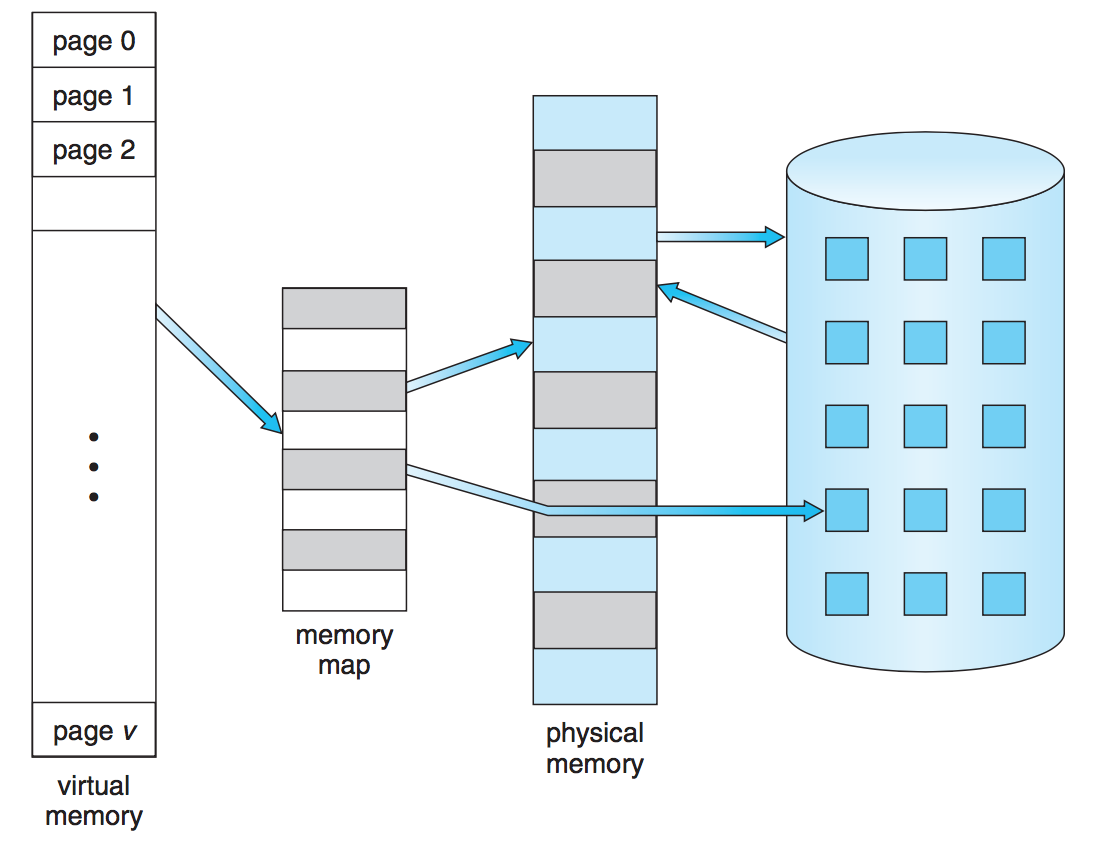
\includegraphics[width=0.5\textwidth]{images/vmem-physmem.png}\\
Virtual memory exceeding the size of physical memory, with some pages on disk~\cite{osc}.
\end{center}

The typical approach is also like that of the cache, which is to use demand paging. A page is loaded into memory only if it is referenced or needed, thus preventing unnecessary disk accesses. This is also called the ``lazy'' approach in~\cite{osc}, though lazy is typically an insult and in this case it is not necessarily bad.  Clearly, we would like to involve disk as little as possible, because disk is, from the perspective of the CPU, extremely slow.

The fact that disk is so slow means we can get into a troublesome state called \textit{thrashing}: the operating system is spending most or all of its time swapping pages in and out of memory and very little actual work can get done.

Apparently, if the NeXT operating system, NeXTStep\footnote{One of the three parents of Mac OS X: the classic Mac OS, BSD [UNIX], and NeXTStep.} were booted on a machine with only 2~MB of RAM instead of the expected 4~MB, the steady state of the system would be a constant level of swapping~\cite{mte241}. This was particularly bad because the most common cause of failure in the NeXT boxes was hard disk drive. But they did have cool magnesium cases, so after they died they at least made impressive conversation pieces and doorstops.

With virtual memory, each memory reference is a six step process~\cite{osc}:

\begin{enumerate}
	\item Check if the memory reference is valid or invalid (just as we have done before).
	\item If the reference is invalid, terminate the program (segmentation fault). If it was valid, but the page referenced is not in memory, we will need to retrieve it.
	\item Find a free frame (or make one by evicting some other page).
	\item Request a disk read (and possibly write) to bring in the new page.
	\item When the disk read is complete, update the records to show the new page is in memory.
	\item Restart the instruction that referenced the page that needed to be brought into memory.
\end{enumerate}

Or, to view this visually:

\begin{center}
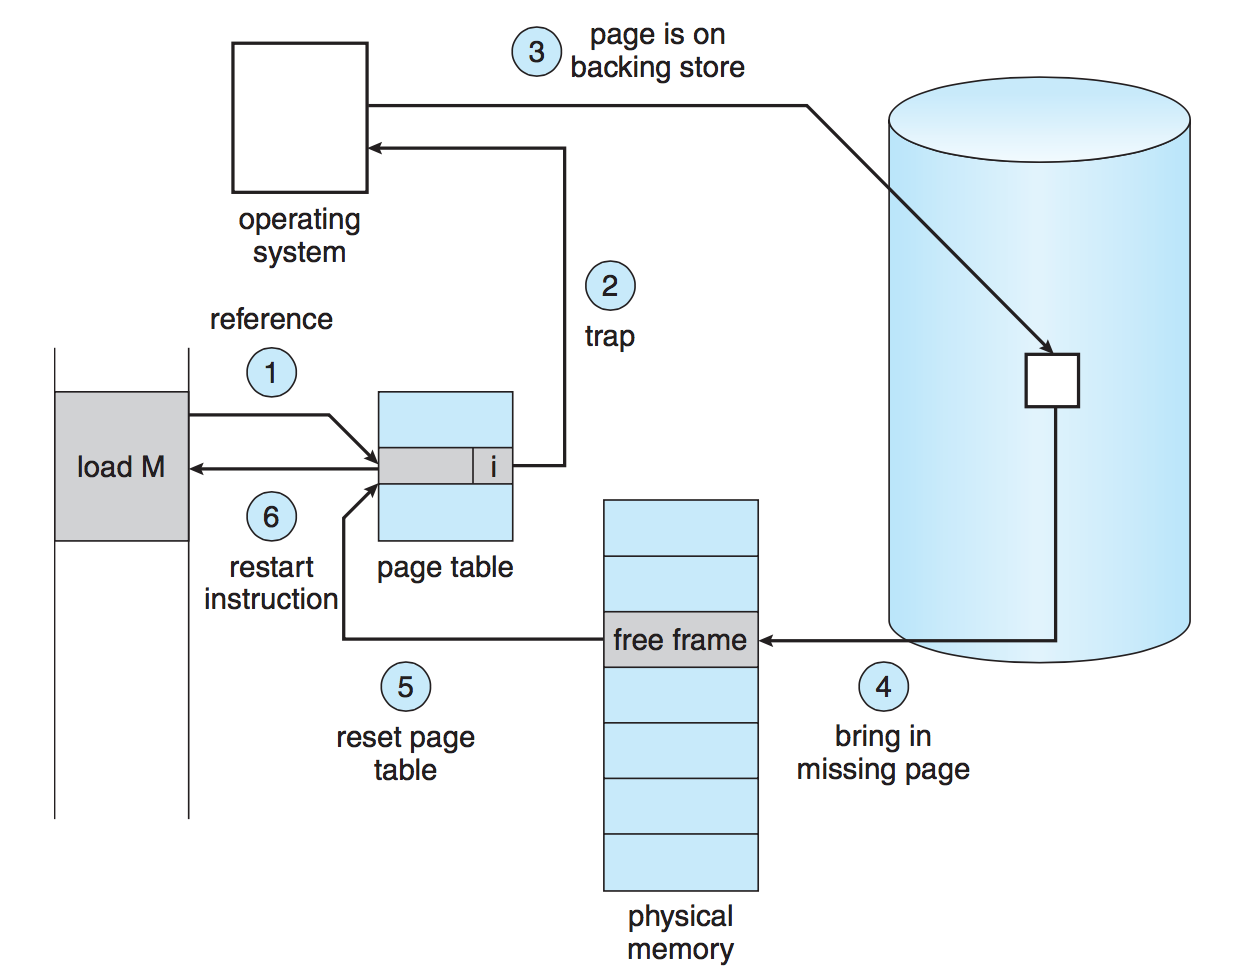
\includegraphics[width=0.7\textwidth]{images/handling-page-fault.png}\\
Handling a page fault~\cite{osc}.
\end{center}

Note that between steps 4 and 5, a significant amount of time will take place while the disk performs a read of the desired page and possibly a write of the page to be evicted if it was modified. While the slow disk operations are going on, the process is blocked on that I/O operation and, in the meantime, the processor can and should be working on something else.

The key requirement in the described workflow is the ability to restart any instruction following the page fault. We save the state of the process, including all the registers and instruction pointer and so on, when the page fault occurs, so we are able to restart the process exactly where it was. The difference is that after the restart, the page needed is in memory and is accessible. A page fault could occur on any memory reference, including fetching the next instruction. If it happens at that time, the fetch operation is done again. If a page fault happens when doing an operation that required fetching an operand, then we fetch and decode the instruction again and then fetch the operand. So a little bit of work may be repeated~\cite{osc}.

Consider the \texttt{ADD} instruction that adds \texttt{A} to \texttt{B} and stores the result in \texttt{C}. First, we must fetch and decode the instruction. That tells us about the two operands, which must be retrieved themselves. Then we can add the two operands, and store the result in the target location. If a page fault occurs when trying to write to \texttt{C}, because that page is not currently in memory, we will restart the instruction. That means back to step one: fetch the \texttt{ADD} instruction again, then get the operands, then perform the addition, and finally write it into the destination location~\cite{osc}.

As we can see, some work is repeated here: fetching and decoding the instruction, as well as taking the operands and doing the addition. This is not a big deal, because the time it takes the CPU to do such an operation is minuscule. CPUs are very good at executing instructions and doing this one a second time is not a big task.

While fetching the page containing \texttt{C} from disk, the page that contains \texttt{A} or \texttt{B} could get swapped out, meaning that the second run of the instruction will also produce a page fault. This is unlikely if using a sane replacement algorithm, because the page with \texttt{A} and \texttt{B} having just been referenced, it is a poor candidate for eviction. But a random page replacement algorithm could result in that behaviour on occasion. While hypothetically possible, it is very unlikely that a system would get stuck on the same instruction forever if the page containing \texttt{A} were constantly replaced in memory and cache by the page containing \texttt{C} and vice versa. But a system vulnerable to this problem would have some very significant design issues, to say the least.

The question is, can every instruction be restarted without affecting the outcome? The answer is no; an example is the situation that occurs when an instruction modifies more than one memory location. If we are moving a block of $n$ bytes, it is possible those bytes will straddle a page boundary\footnote{Some CPUs and operating systems have boundary issues and take this kind of thing a bit more seriously, requiring alignment of data structures to byte and block boundaries... others don't seem to mind at all.}, either at the source or destination. We would like to avoid this situation, because the move operation may not be easily restarted if the source and destination overlap (i.e. the source is modified). One is for the CPU to try to access the start and end addresses before the move begins; if one of the pages needed is not in memory, the page fault is triggered before any data is changed, so we can be sure the move will succeed when it actually starts. Another solution is temporary registers to hold overwritten location; if a page fault occurs, then the temporary data is restored so the instruction may be restarted without affecting the operation's correctness~\cite{osc}.

\subsection*{Virtual Memory Performance}

As we have already seen, finding something in the cache is significantly faster than having to go to main memory. Retrieving something from disk is dramatically slower, but computing how long it takes to retrieve a given page will follow the same principle. Recall from earlier the effective access time formula:

\begin{center}
	Effective Access Time = $ h \times t_{c} + (1 - h) \times t_{m}$
\end{center}

Where $h$ is the hit rate, $t_{c}$ the time to retrieve a page from cache, and $t_{m}$ is the time to retrieve it from memory. If we replace the terms $t_{c}$ and $t_{m}$ with $t_{m}$ and $t_{d}$ (time to retrieve it from disk) respectively, and redefine $h$ as $p$, the chance that a page is in memory, we can get an idea of the effective access time in virtual memory: 

\begin{center}
	Effective Access Time = $ p \times t_{m} + (1 - p) \times t_{d}$
\end{center}

And just while we're at it, we can combine the caching and disk read formulae to get the true effective access time for a system where there is only one level of cache:

\begin{center}
	Effective Access Time = $ h \times t_{c} + (1 - h) ( p \times t_{m} + (1 - p) \times t_{d})$
\end{center}

This is good, but what is $t_{d}$? This is a measurable quantity so it is possible, of course, to just measure it\footnote{One of my favourite engineering sayings is ``Don't guess; measure.''}. We expect $p$ to be small if our paging algorithm is any good. But what needs to take place to handle a page fault (miss) is~\cite{osc}:

\begin{enumerate}
	\item Trap to the operating system.
	\item Save the user registers and process state.
	\item Identify this interrupt as a page fault.
	\item Check that the page reference was legal. 
	\begin{enumerate}
		\item If so, determine the location of the page on disk.
		\item If not, terminate the requesting program. Steps end here.
	\end{enumerate}
	\item Figure out where to place the page in memory (use our replacement algorithm).
	\item Is the frame we have selected currently filled with a page that has been modified? 
	\begin{enumerate}
		\item If so, schedule a disk write to flush that page out to disk. The disk write request is placed in a queue.
		\item If not, go to step 11.
	\end{enumerate} 
	\item Wait for the disk write to be executed. The CPU can do something else in the meantime, of course.
	\item Receive an interrupt when the disk write has completed.
	\item Save the registers and state of the other process if the CPU did something else.
	\item Update the page tables to reflect the flush of the replaced page to disk. Mark the destination frame as free.
	\item Issue a disk read request to transfer the page to the free frame.
	\item As before, while waiting, let the CPU do something else.
	\item Receive an interrupt when the disk has completed the I/O request.
	\item Save the registers and state of the other process if the CPU did something else.
	\item Update the page tables to reflect the newly read page.
	\item Restore the state of and resume execution of the process that encountered the page fault, restarting the instruction that was interrupted.
\end{enumerate}

The slow step in all of this, is obviously, the amount of time it takes to load the page from disk. According to~\cite{osc}, restarting the process and managing memory and such take something like 1 to 100~$\mu$s. A typical hard drive in their example has a latency of 3~ms, seek time (moving the read head of the disk to the location of the page) is around 5~ms, and a transfer time of 0.05~ms. So the latency plus seek time is the limiting component, and it's several orders of magnitude larger than any of the other costs in the system. And this is for servicing a request; don't forget that several requests may be queued, making the time even longer.

Thus the disk read term $t_{d}$ dominates the effective access time equation. If memory access takes 200~ns and a disk read 8~ms, we can roughly estimate the access time in nanoseconds as $(1-p) \times 8~000~000$. 

If the page fault rate is high, performance is awful. If performance of the computer is to be reasonable, say around 10\%, the page fault rate has to be very, very low. On the order of $10^{-6}$. 

And now you also know why solid state drives, SSDs, are such a huge performance increase for your computer. Instead of spending time measured in the milliseconds to find a page on disk, SSDs produce the data much quicker, with times that look more like memory reads.

We have not yet covered file systems, but files tend to come with a bunch of overhead for file creation and management. To avoid this, the system usually has a ``swap file'' which is just one giant file or partition of the hard drive. The system can get better performance by just dealing with the swap file as one big file (block) and not tiny individual files~\cite{osc}.

\subsection*{Copy-on-Write}
Recall that in UNIX we create a new process with a call to \texttt{fork()} and that this creates an exact duplicate of the parent process. That process may replace itself with the \texttt{exec()} system call immediately. Thus it seems like it might be a waste of time to copy the memory space of the parent if the child is just going to throw it away immediately. What UNIX systems do is use the \textit{copy-on-write} technique: the parent and child share the same pages, but they are marked as copy-on-write~\cite{osc}.

If there is immediately an \texttt{exec()} invocation then the new memory pages for the child are brought in and the unnecessary work is avoided. But suppose the child is to remain a clone of the parent.

Initially, all pages are shared but marked. As soon as either the parent or child attempts to modify a page, a copy of the page is made and the modification is then applied to the new copy of the page. All unmodified pages remain shared, but only the pages that are actually modified will be copied, so there is no unnecessary copying.

Some versions of UNIX, notably Solaris and Linux, have a system call \texttt{vfork()} which skips the copy-on-write procedure. The parent process is suspended and the child process uses the memory space of the parent~\cite{osc}. So any alterations the child makes will be visible to the parent when it resumes. Thus this is potentially dangerous, as the child can wreak a whole bunch of havoc. This is efficient if the intention is to immediately \texttt{exec()} and get a new memory space.

\bibliographystyle{alpha}
\bibliography{254}


\end{document}